\documentclass{ctexart}

\title{软件工程}

\usepackage{graphicx}

\begin{document}
\maketitle

\section{介绍}
\paragraph{生命周期地看待} 软件不是写完就完了, 而是需要持续的维护.
\paragraph{过程评估} 即使软件没有完成, 也可以在过程中评估软件.
\pagebreak{项目产出} 项目的产出除了可用的程序, 还有如文档.
\paragraph{人月神话} 软件开发中, 不是人越多就开发越快, 相反可能更多的中途加入的人会拉慢进度.
\paragraph{开发和客户交流} 客户需要不断的和开发交流, 以修正轨迹和提供更精确的方向指导.

\section{持续集成和git}
    系统可能随时变化, 预测式的开发已经不合时宜了.

\section{代码风格}


\pagebreak
\section{重构}
    \begin{figure}[ht!]
        \centering
        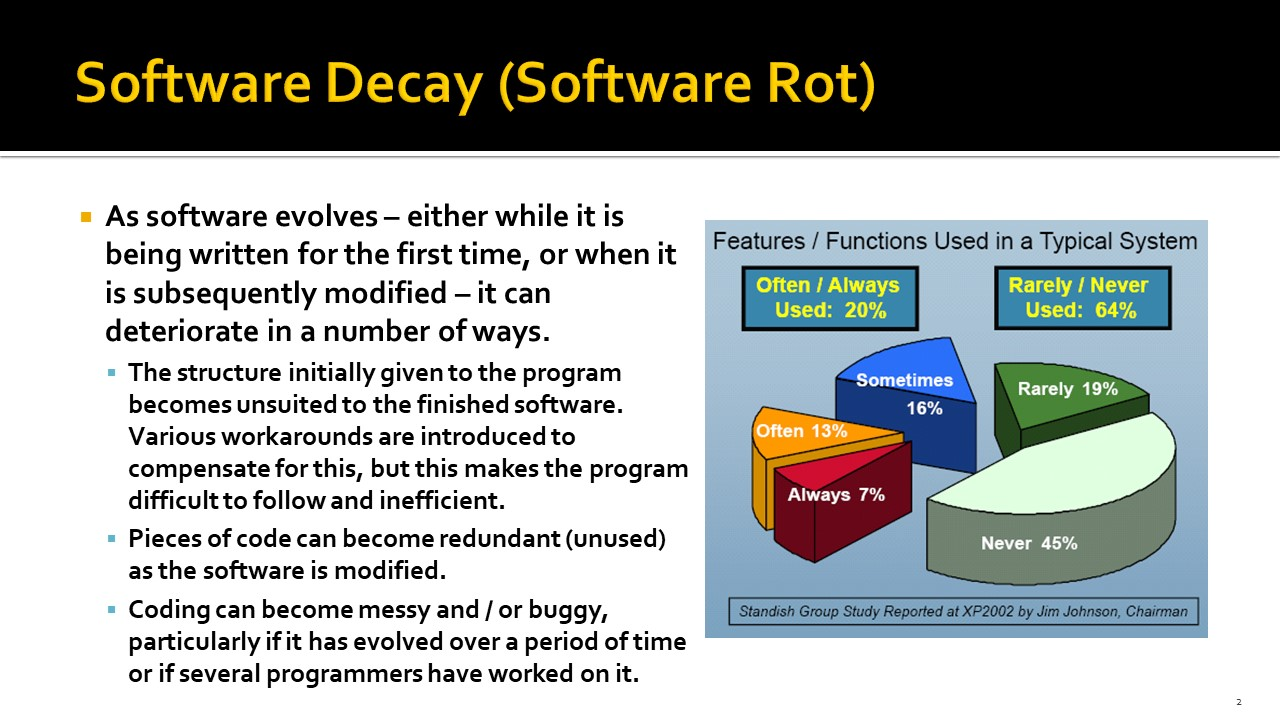
\includegraphics[width=\textwidth, height=\textheight, keepaspectratio]{refactor-1.jpg}
        \caption{Software Rot现象}
    \end{figure}

    \begin{figure}[ht!]
        \centering
        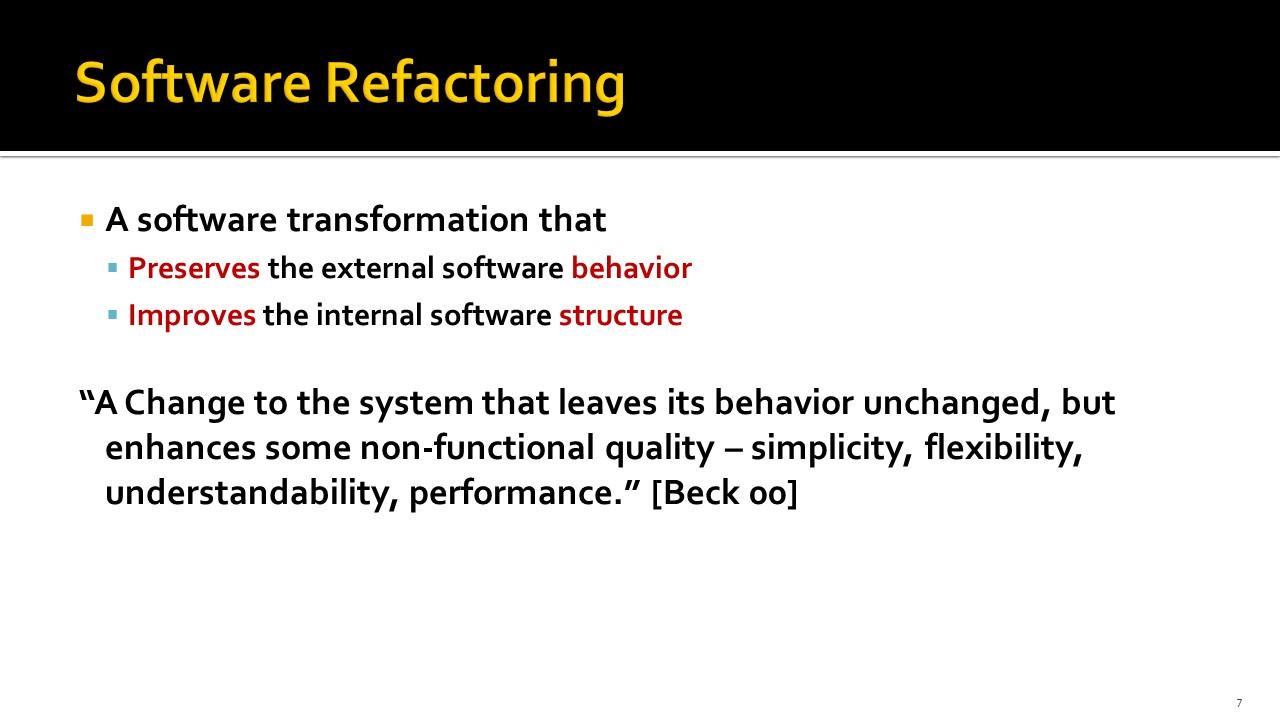
\includegraphics[width=\textwidth, height=\textheight, keepaspectratio]{refactor-2.jpg}
        \caption{何谓Refactoring}
    \end{figure}

    \begin{figure}[ht!]
        \centering
        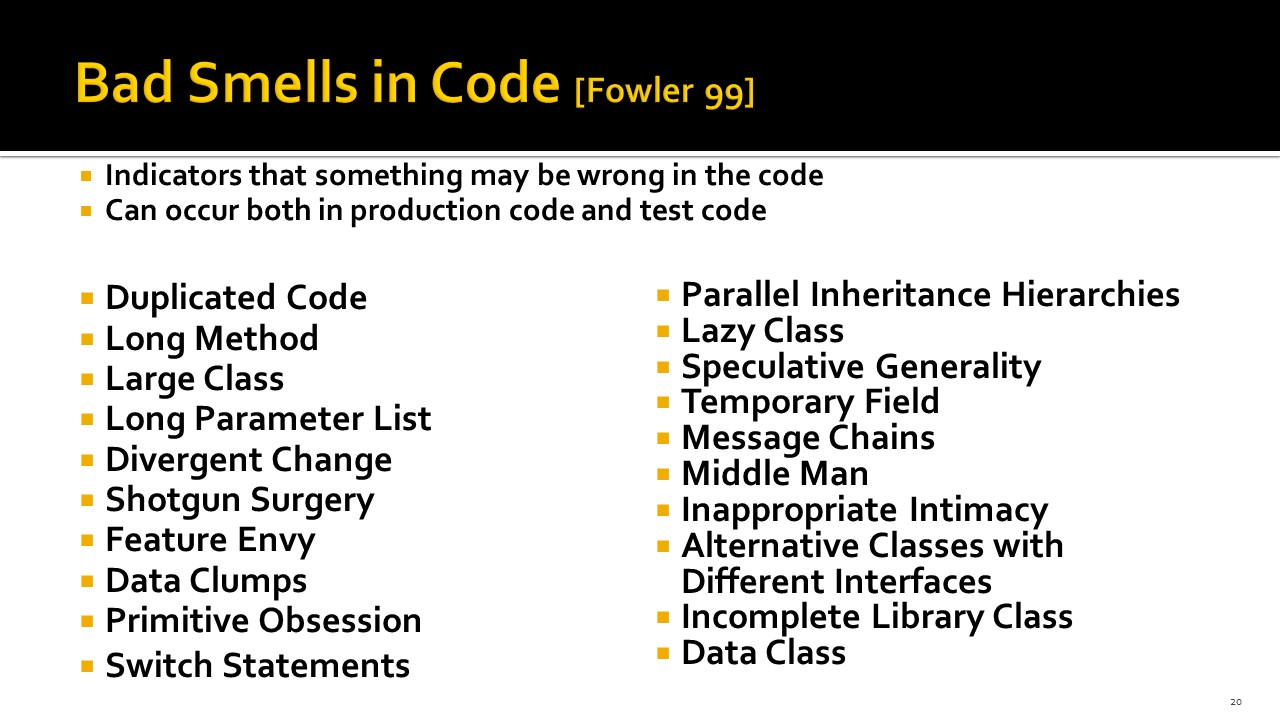
\includegraphics[width=\textwidth, height=\textheight, keepaspectratio]{refactor-3.jpg}
        \caption{常见的Code Smell}
    \end{figure}

    \begin{figure}[ht!]
        \centering
        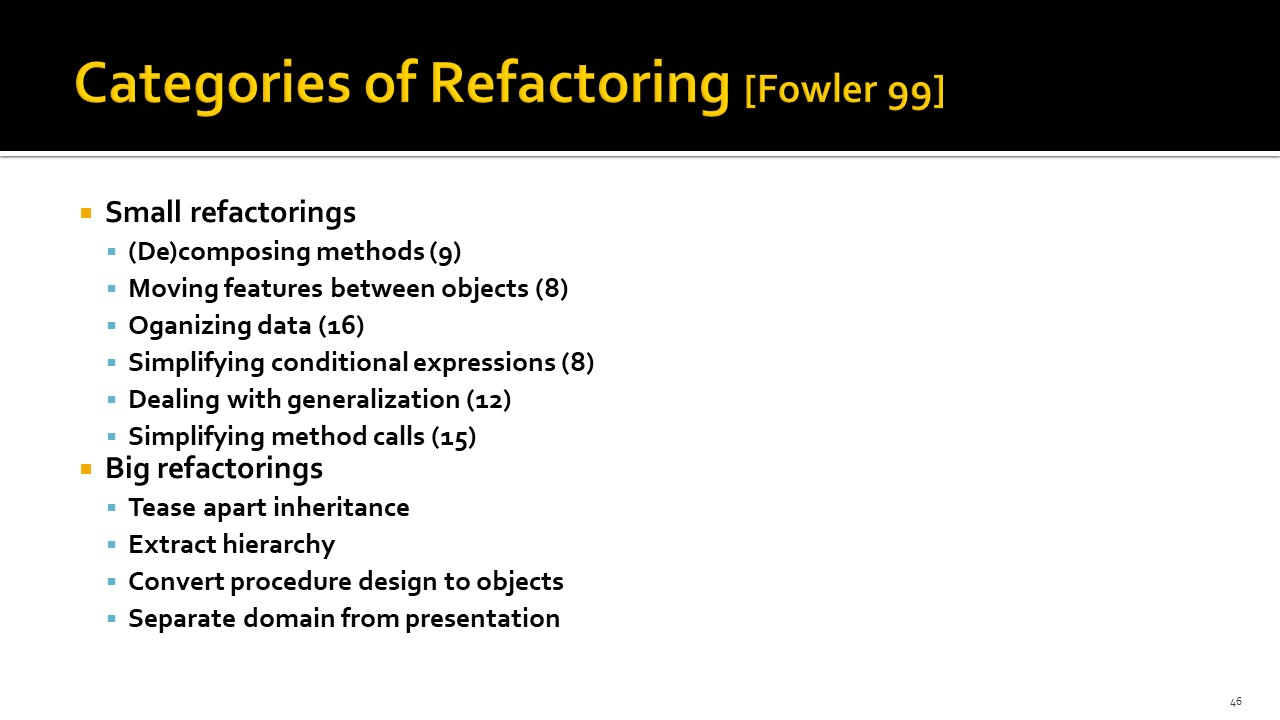
\includegraphics[width=\textwidth, height=\textheight, keepaspectratio]{refactor-4.jpg}
        \caption{常见的Refactor方法}
    \end{figure}

\section{测试}
    测试: 希望找到错误.
    好的测试是容易找到错误的测试.\par
    基本原则是, 测试是不可穷尽的.
\paragraph{测试样例} 指定输入, 输出, 以及可能的执行前置条件etc.
\subsection{分类}
    \begin{description}
        \item[白盒测试] 已知要测试的代码. 是基于代码测试的, 测试功能是代码的子集.\\
            包含控制流覆盖率和数据流覆盖率;
        \item[黑盒测试] 已知要测试的特性, 是基于规格测试的, 测试功能是规格的子集.\\
            包含需求覆盖率
    \end{description}
    考虑测试韦恩图, 有集合$S$表示规格, $P$表示程序, $T$表示测试.
    白盒测试是$T \subseteq P$; 黑盒测试是$T \subseteq S$.
\subsection{控制流测试}
\paragraph{Statement Coverage}
    C0测试; 所有语句都必须被测试覆盖.\par
    方法: 在控制流图中找到覆盖所有语句 (即覆盖所有节点) 的路径 (可能的话需要路径集合), 寻找输入适配此路径.
\paragraph{Decision Coverage}
    C1测试; 所有if语句的条件必须测试过true和false.\par
    方法: 寻找覆盖所有分支 (每个节点的每条出边必须被覆盖) 的路径集合, 寻找输入适配路径集合.
\paragraph{Predicate Converage}
    C1P测试; 所有if语句的条件中每个原子条件必须测试过true和false.\par
    方法: 将if的复合条件改写成嵌套if之后看.
\paragraph{Multiple Condition Coverage}
    CMCC测试; \emph{每个复合条件}中所有原子条件的组合都被测试. 组合会有依赖关系所以不一定是$2^n$种路径.\par
    方法: 同C1P测试, 只是需要更多路径.
\paragraph{All Path Coverage}
    C$\infty$测试; \emph{整个程序}中所有原子条件的组合都被测试, 即所有路径都被测试.\par
    通常在有循环时时不可行的, 或者在条件互斥时也不可行 (某一条路径不存在对应的输入).
\paragraph{cyclomatic complexity (McCabe complexity)}
    覆盖所有控制语句 (C0测试) 需要的最少的测试例数. 其等于流图中, 决策的数量加1.
\paragraph{Independent Path}
    有向图中的独立路径. 数目等于 cyclomatic complexity.

\subsection{数据流测试}
    不正常的数据行为: \begin{itemize}
        \item (dd) 定义之后, 引用前重定义
        \item (ur) 未定义时引用
        \item (du) 定义后未引用
    \end{itemize}
    数据流分析分为静态和动态, 以是否执行原代码为准.
\paragraph{DU链} $[X, S, S']$的形式, $S$, $S'$是语句,
    $S$定义而$S'$引用$X$, 并且$S$的定义在$S'$是存活的.
\paragraph{数据流图} 将数据的引用分为计算引用 (C-uses) 和条件引用 (P-uses),
    基本结构类似流图, 但是结点是计算引用, 边与条件引用挂钩.
\paragraph{覆盖度量} 包含 All paths (通常不可能),
    All DU paths, All Edges (通常最低要求)等.

\subsection{黑盒测试}
\paragraph{基本思想} 将输入空间分成多个等价类, 每个等价类对于程序来说是等价的, 从``发现错误''的角度.
\paragraph{强弱测试} 强测试即, 可能有多个无效的输入, 弱测试即, 只有一个输入时无效的.
\paragraph{普通鲁棒测试} 普通测试只覆盖有效数据, 鲁棒测试还覆盖无效数据.\par
    普通鲁棒测试和强弱测试都是EP测试.
    \begin{figure}[ht!]
        \centering
        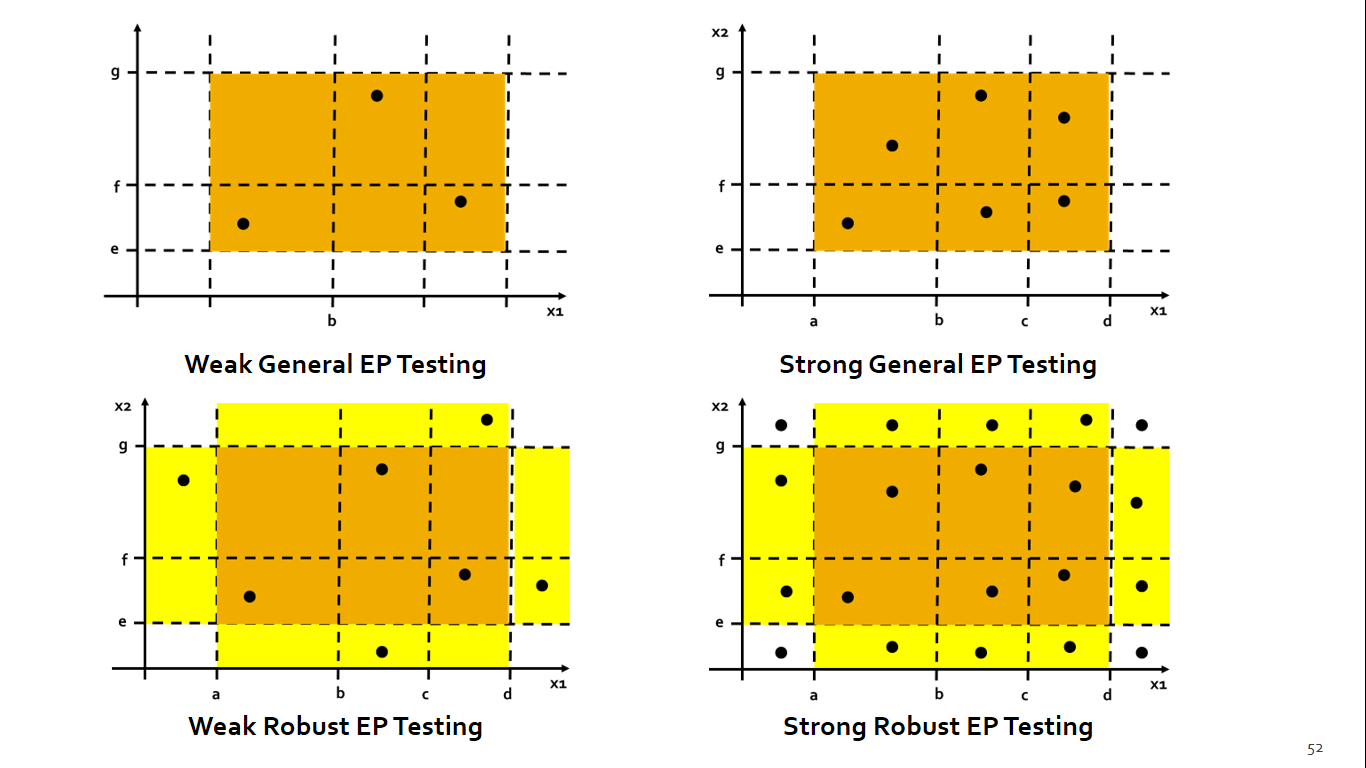
\includegraphics[width=\textwidth, height=\textheight, keepaspectratio]{eptest.png}
        \caption{EP测试的例子}
    \end{figure}

\paragraph{边界值分析} 通常问题都是在输入在输入域边界时出现的.
    因此, 选择数据时, 不是随机在数据空间选择, 而是在空间边界选择.
    同时也从输出域中寻找数据.\par


\section{xUnit}
\paragraph{测试的重要性} 有``错误率恒定定律'', ``规模代价平方定律'', 所以需要
    尽可能早地发现错误,并在尽量小的范围内定位并修复错误.
\paragraph{测试驱动开发}
    开发新特性之前先写测试 (此时必定失败). 能够使得开发人员专注于需求.
\paragraph{基本架构}
    \begin{figure}[ht!]
        \centering
        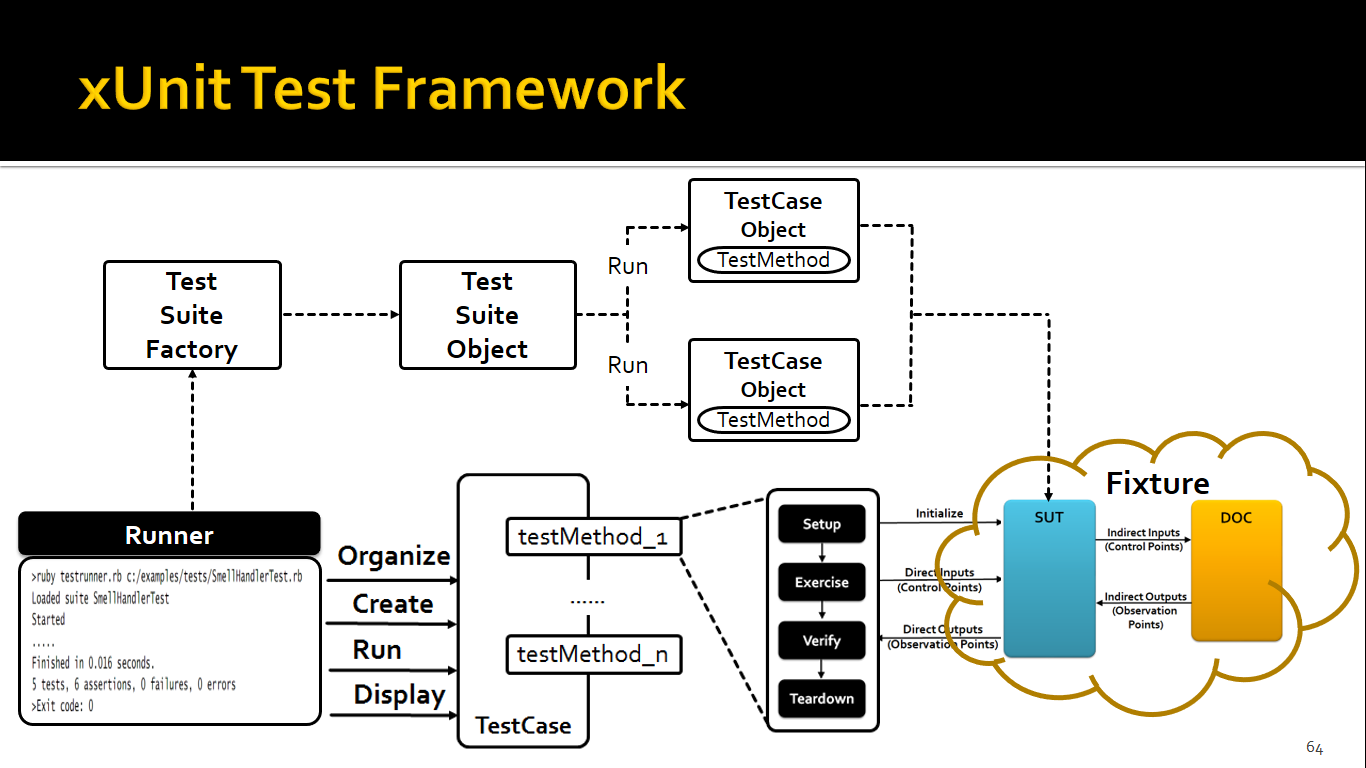
\includegraphics[width=\textwidth, height=\textheight, keepaspectratio]{xunit-1.png}
        \caption{xunit基本架构}
    \end{figure}
\paragraph{setup / teardown} 应当delegate inline setup / teardown;
\paragraph{verification} 分为behavioural, state, delta etc.
\paragraph{test doubles} 需要依赖的系统 (DOC) 不可用或者不方便. 可以用一个假的DOC, 也方便监控.\par
    如Dummy Object: 假的值. Test Stub: 提供indirect input. Test Spy / Mock Object: 检查indirect output.
    
\section{系统测试}
\paragraph{测试分类}\begin{itemize}
        \item 单元测试, 单个模块的功能实现
        \item 集成测试, 模块之间的接口测试
        \item 系统测试, 包含其他系统, 如硬件等
    \end{itemize}
\subsection{集成测试}
    不要一次测试所有单元的继承, 而是增量式地, 一部分一部分测试然后再接起来.
\paragraph{Top-down 集成}
    从顶层单元开始. 未计入的底层用 Test Stubs 代替.\par
    问题是, 需要写大量的stub.
\paragraph{Bottom-down 集成}
    从底层开始. 需要一个控制器 (test driver), 用于假装上层单元.\par
    问题是, 最重要的主逻辑是最后测试的.

\subsection{效率测试}
    性能: 响应时间; 吞吐量; 数据容量; 实时性.\par
    测试: 负载测试 (load testing): 在一个指定的负载下;
        压力测试 (stress testing): 极限负载;
        soak testing: 在指定负载下的\emph{持续}表现;
        spike testing: 突然增加负载;
        configuration testing: 确定配置对于系统表现的影响.\par

\section{需求工程}
    需求将用户的目标和期望转化为工程师的规格说明.
\paragraph{用户}
    需要确定给谁做, 做什么, \emph{不做什么}.
\paragraph{需求分层} \begin{enumerate}
        \item 业务需求 -> 愿景和范围文档
        \item 用户需求 -> 用户需求文档
        \item 软件需求 -> 软件需求规格说明
    \end{enumerate}
\paragraph{需求建模泳道图}
    \begin{figure}[ht!]
        \centering
        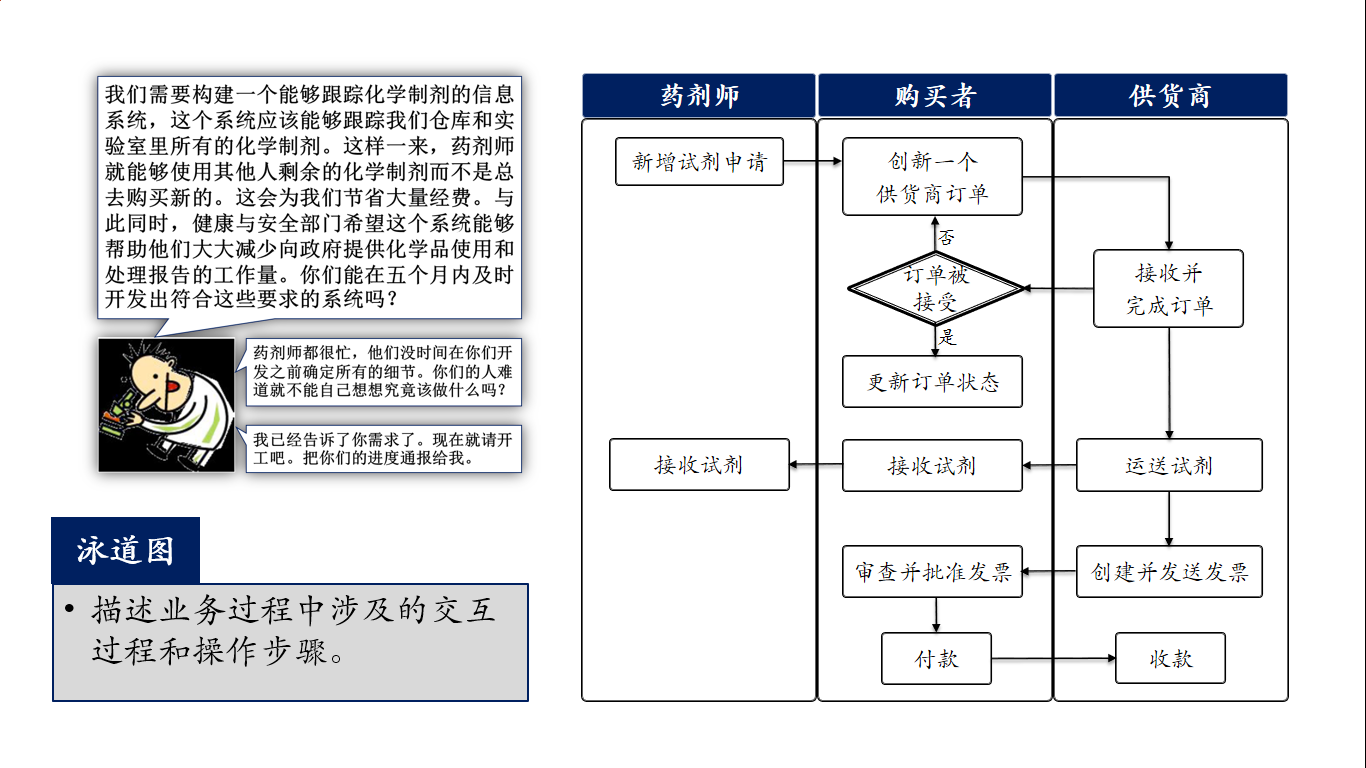
\includegraphics[width=\textwidth, height=\textheight, keepaspectratio]{lane.png}
        \caption{泳道图}
    \end{figure}
\paragraph{数据流图}
    分层需要满足平衡规则, 即不漏不多.
\paragraph{判定方法}
    \begin{figure}[ht!]
        \centering
        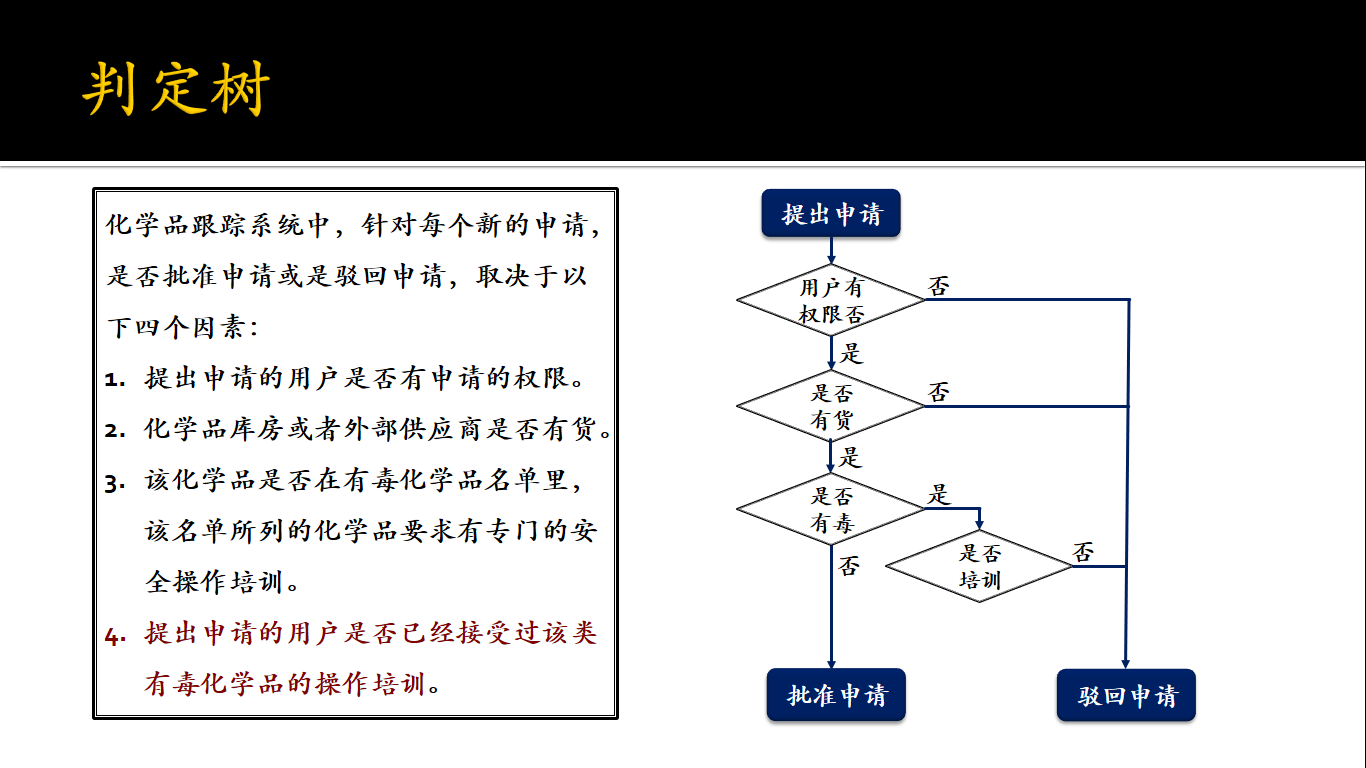
\includegraphics[width=\textwidth, height=\textheight, keepaspectratio]{pred-tree.png}
        \caption{判定树方法}
    \end{figure}
    
    \begin{figure}[ht!]
        \centering
        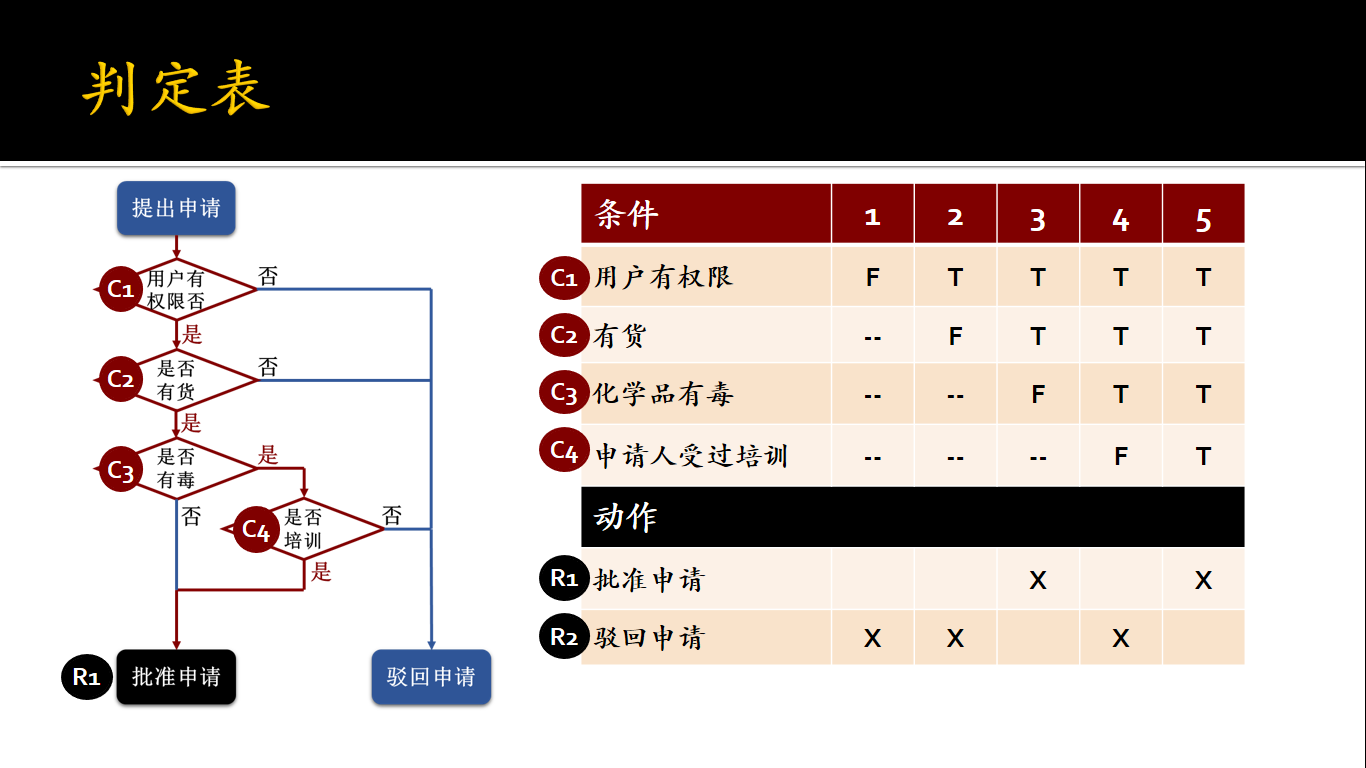
\includegraphics[width=\textwidth, height=\textheight, keepaspectratio]{pred-tbl.png}
        \caption{判定表方法}
    \end{figure}
\paragraph{软件需求规格说明 SRS}
    应当足够详细. 效率需要可测.\par
    良好的SRS, 可验证, 每个需求是为了一个业务目标, 可测并且有界.\par
    [条件] [主体] [动作] [客体] [对某个参数的约束] [约束的值]\par
    需求应当正确, 准确, 无二义性, 量化的, 并且覆盖所有情况\par
    需求不应当随便变更, 变更前应当经过评估.\par

\section{UML}
\paragraph{基本架构} 4+1 视图 \begin{itemize}
        \item Design
        \item Implementation
        \item Process
        \item Deployment
        \item *** Use case ***
    \end{itemize}
\paragraph{用例图}
    \begin{figure}[ht!]
        \centering
        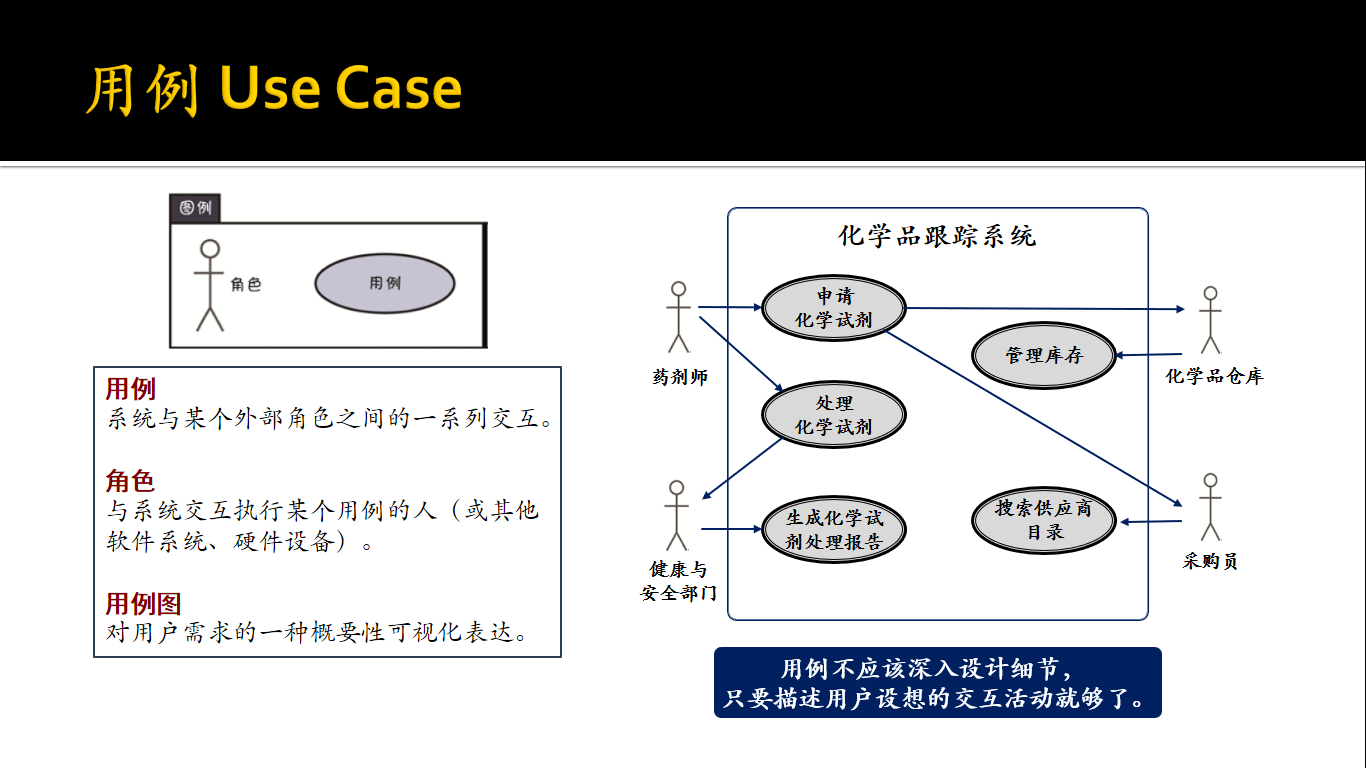
\includegraphics[width=\textwidth, height=\textheight, keepaspectratio]{usecase.png}
        \caption{用例图例子}
    \end{figure}
    Actor: 一个和系统交互的实体.\par
    use case: 系统的主要的功能.\par
\paragraph{Class Diagram}
\paragraph{Sequence Diagram}
    不一定, 但通常是一个use case之内的描述.\\
    从实体和时间两个维度定义了系统的行为.\par
    \begin{figure}[ht!]
        \centering
        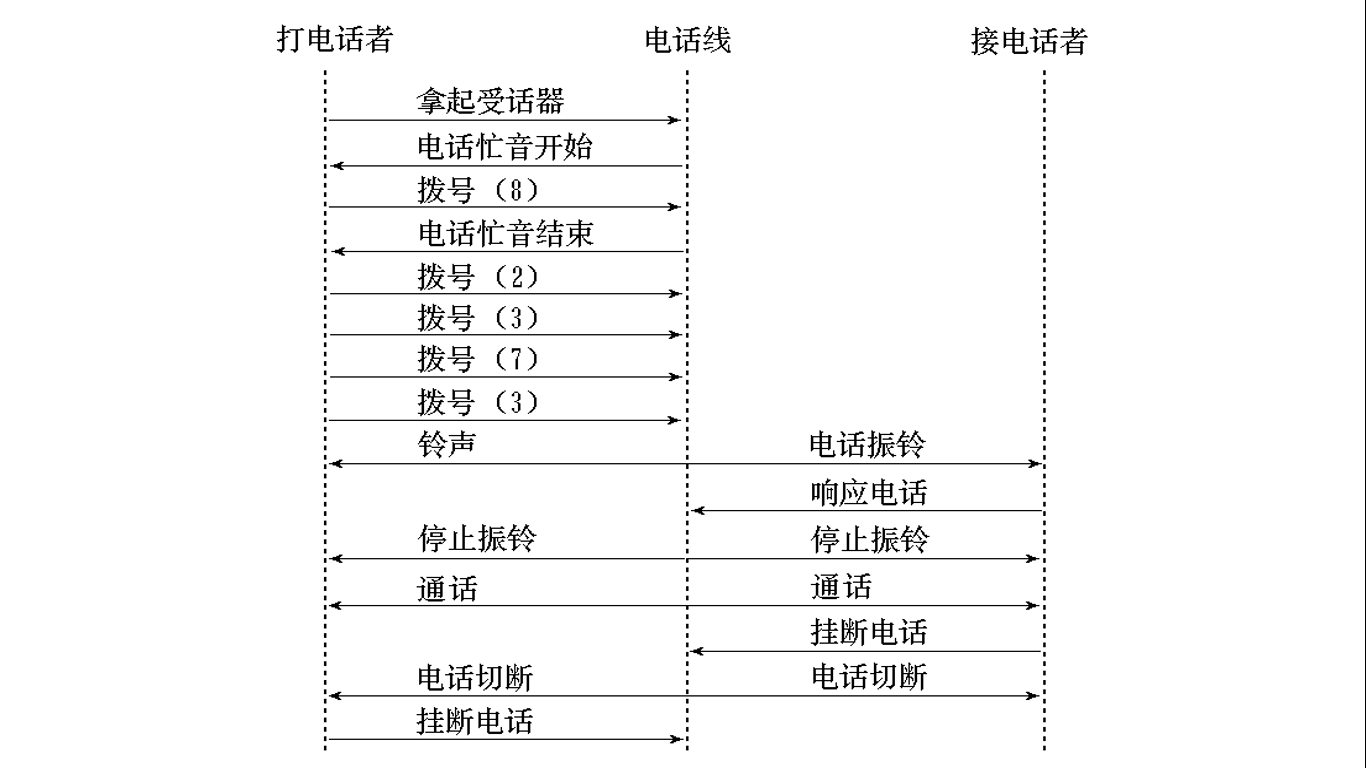
\includegraphics[width=\textwidth, height=\textheight, keepaspectratio]{seqdiag.png}
        \caption{Sequence Diagram例子}
    \end{figure}
    并且class diagram也是sequence diagram的一部分, 如
    \begin{figure}[ht!]
        \centering
        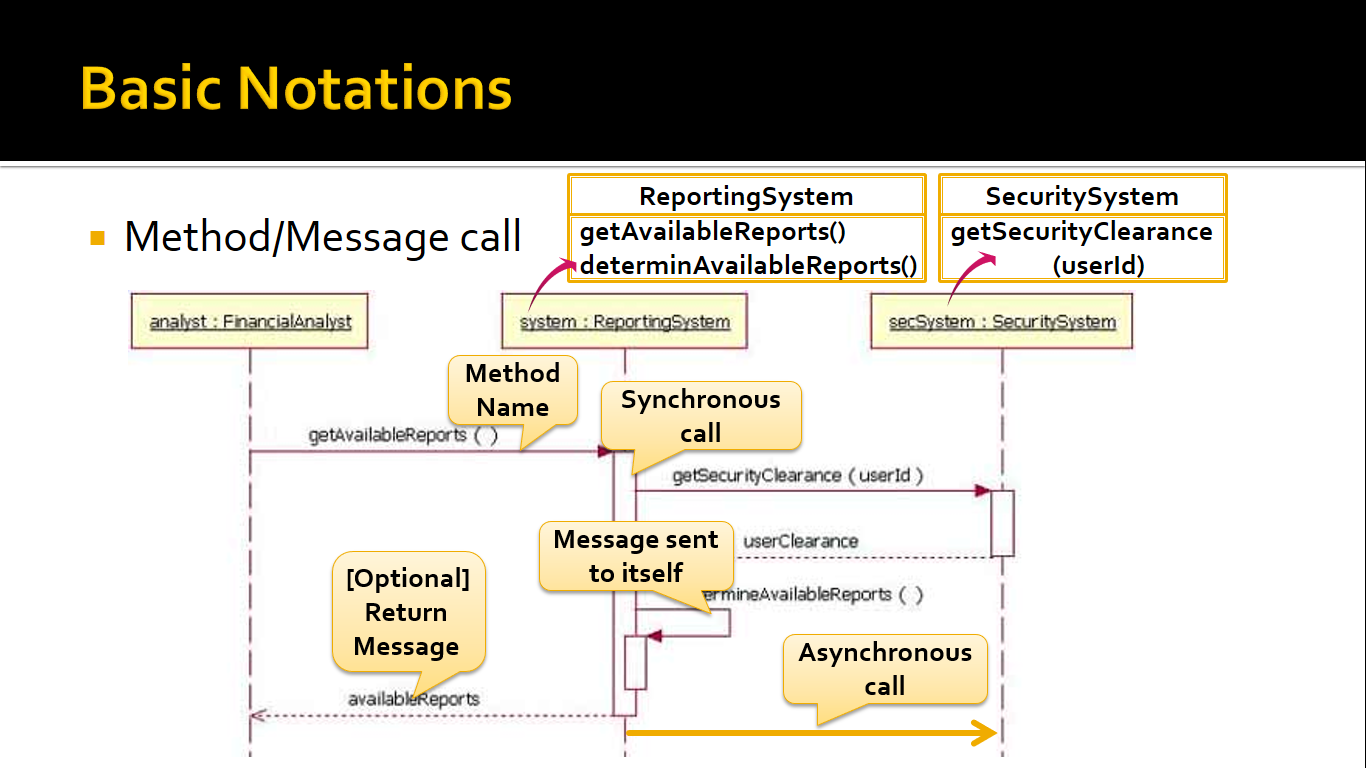
\includegraphics[width=\textwidth, height=\textheight, keepaspectratio]{seqdiag1.png}
        \caption{Class Diagram例子}
    \end{figure}
    方法就是, 将原需求拆成一系列的 (subject) {action} (object).
    subject和object统称物, 每个物形成一条数显, 按照正确的顺序,
    从subject有一个到object的横箭头, 上面写action.\par
    如数据, 电话线等等都算``物''. 一个例子如图.
    \begin{figure}[ht!]
        \centering
        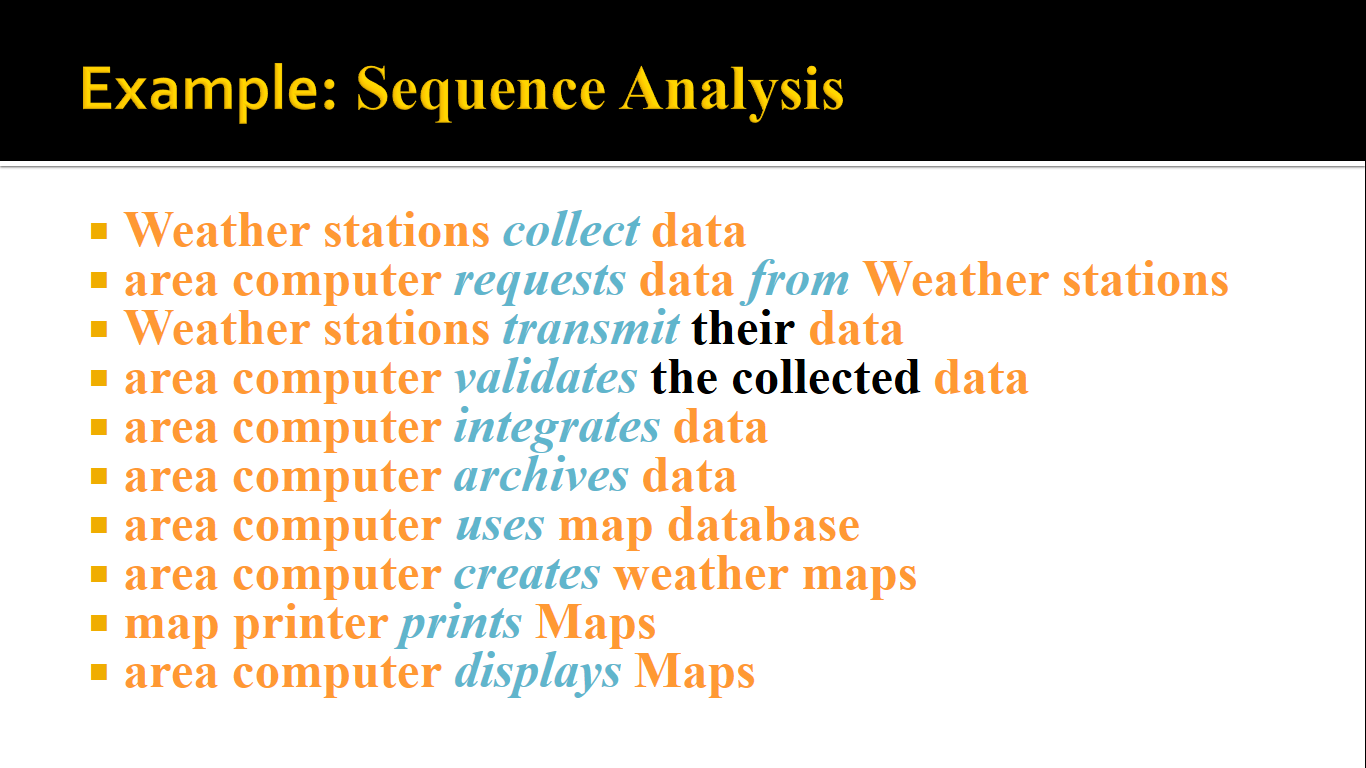
\includegraphics[width=\textwidth, height=\textheight, keepaspectratio]{seqdiag2.png}
        \caption{构造sequence diagram}
    \end{figure}
    \begin{figure}[ht!]
        \centering
        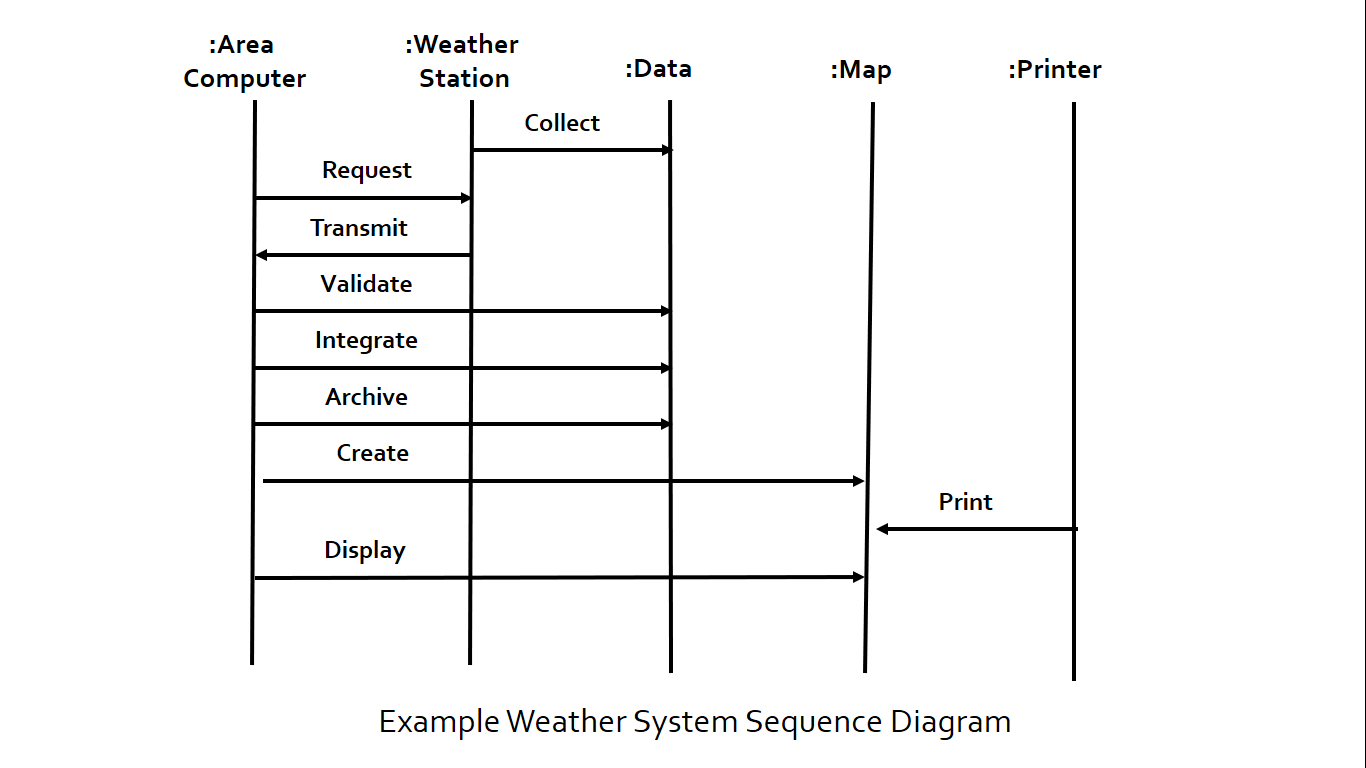
\includegraphics[width=\textwidth, height=\textheight, keepaspectratio]{seqdiag3.png}
        \caption{构造sequence diagram}
    \end{figure}

\section{软件设计}
\paragraph{设计原则} 模块化, KISS, 面向变化和重用, seperation of concerns.
\paragraph{KISS} 简化代码, 简化架构 (中间件总线), 即插即拔.
\paragraph{模块化} 设计时候考虑 coupling 和 cohesion.
    要弱耦合, 强内聚.
\paragraph{seperation of concerns} 每个程序元素做一个且仅一个事情.
\paragraph{面向变化} 封装可能变化的, 保持接口不变; 允许动态绑定.
\paragraph{面向重用} 

\section{架构}
    架构和功能不是分离的, 架构影响软件质量.\par
\paragraph{性能}
    包含 (并发性, 速度etc), 解决方法有队列, 均衡负载等
\paragraph{可用性}
    定义为足够长的时间段内可用时间的比例.\par
    对于硬件, 可以用冗余投票提高可用性.\par
    对于软件, 可以N版本编程. 但不能避免错误, 如多个团队犯了同样的错误, 或者尤其是规格中的错误.
\paragraph{可修改性}
    将旧的开发框架做成product line, 在新的开发中使用. 并且同时也不断优化旧的开发框架.
\paragraph{架构风格}
    \begin{itemize}
        \item 事件驱动. 可以直接用callback管理.
                也可以利用间接方法: 实现广播模型, 在总线上广播; 或者采用中断处理方法.
        \item 管道和filter. 每个模块的输入通过模块变换到输出, 一个模块的输出接到另一个模块的输入上.
        \item 分层架构. 如OSI RefModel.
        \item 仓库. 一个中心仓库保存所有子系统需要的数据.
    \end{itemize}
\paragraph{分布式架构风格}
    分布式的有C/S风格和P2P风格.
    \begin{figure}[ht!]
        \centering
        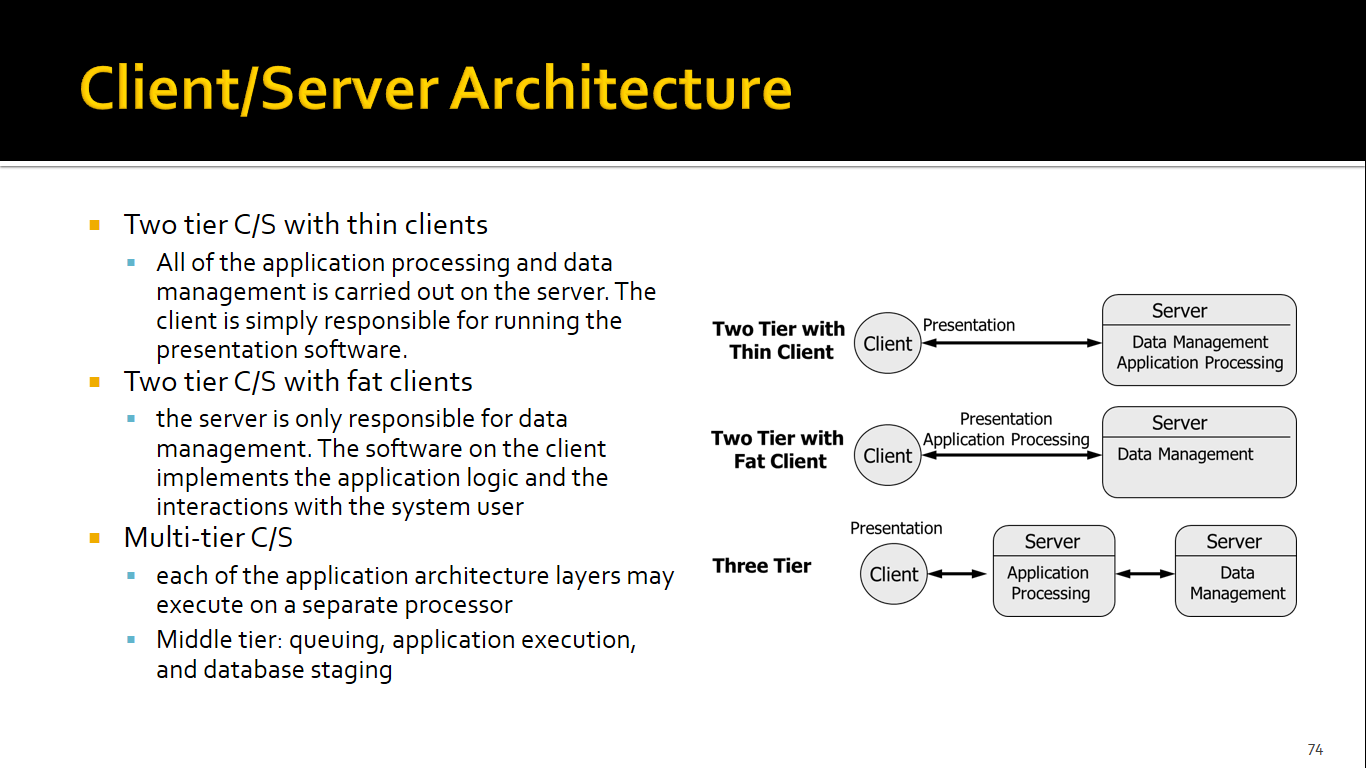
\includegraphics[width=\textwidth, height=\textheight, keepaspectratio]{csarch.png}
        \caption{C/S的架构风格}
    \end{figure}
\paragraph{SOA} Service oriented architecture. C/S设计, 但是更强调软件部件间的解耦合.
\paragraph{Micro-Service} 一个应用是一系列小而专一的服务组成的. 服务自己是一个进程,
    其间通过轻量级的方式 (如HTTP API) 通信. 
\paragraph{Web应用架构} REST, 服务器集群\ldots


\section{质量管理}
\paragraph{critical system}
    可靠性要求极高的系统, 甚至允许采用不经济的手段保证可靠性.
\paragraph{错误种类} \begin{description}
        \item[fault] 错误可能的源头
        \item[error] 到达服务接口的fault
        \item[failure] 导致服务出现错误的error
    \end{description}
\paragraph{V\&V} Verification: 是否符合规格; Validation: 是否符合客户期望.
\paragraph{inspection}
    包括code review, formal inspection.
\paragraph{cleanroom computing}
    目的是完全避免错误.
    包含 peer review; 增量开发等等.\par

\section{项目管理}
\paragraph{团队} 需要团结etc.
\paragraph{工作分解} 如responsibility assignment matrix.
\paragraph{任务调度} 寻找什么任务是不能拖延的:
    使用关键路径方法, 通过earliest和latest来完成.
\paragraph{甘特图} 如图.
    \begin{figure}[ht!]
        \centering
        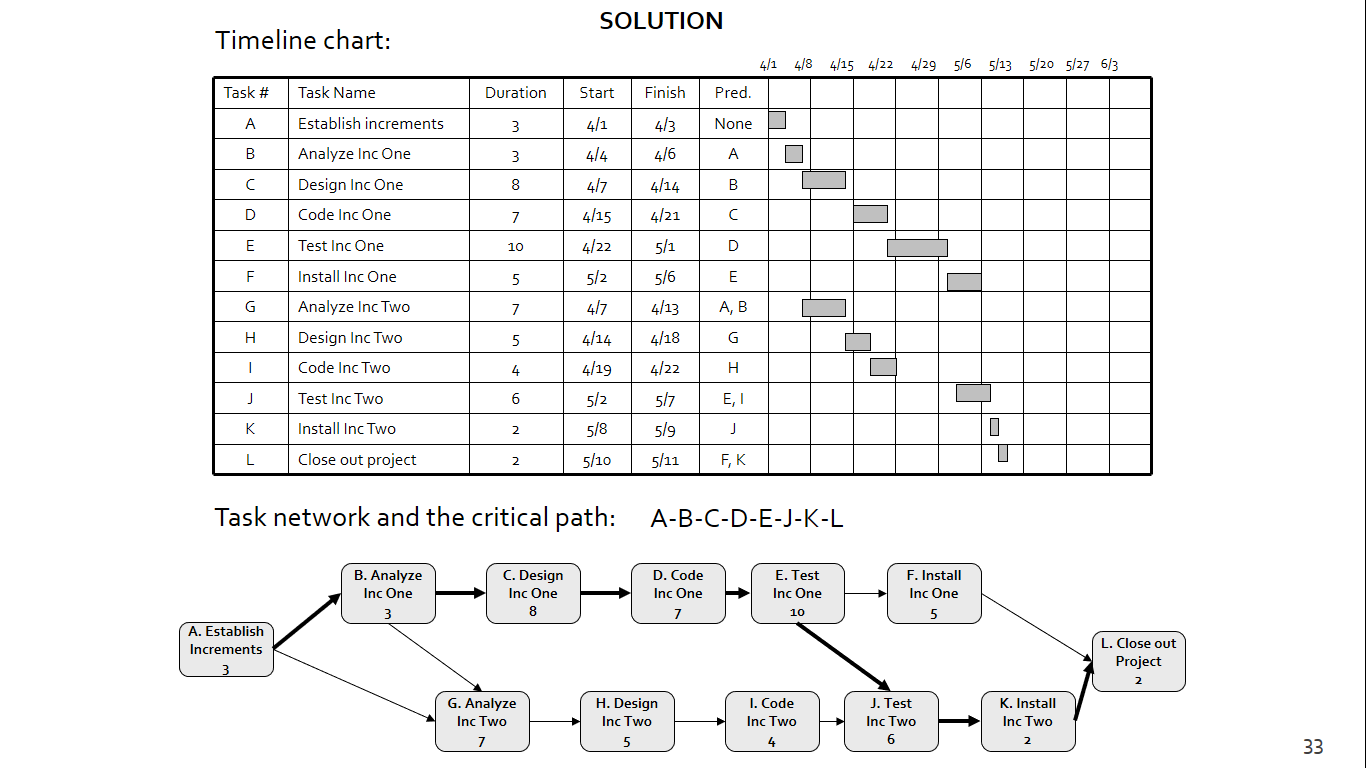
\includegraphics[width=\textwidth, height=\textheight, keepaspectratio]{gantt.png}
        \caption{甘特图}
    \end{figure}
\paragraph{风险管理} 有``救火队员''的风险处置方法, 以及预先做好准备的风险管理.
    RMMM: Risk Mitigation, Monitoring, Management.

\section{Software Process}
    软件的质量被其过程管理的质量控制.
\paragraph{软件开发模型}
    \begin{itemize}
        \item 瀑布模型. 需求确定, 一步一步地完成. 不能很好的适应需求改变.
        \item 增量模型. 一部分一部分地开发, 每次都只分析这一部分的需求.
        \item 原型模型. 开发过程中, 利用原型和客户交流, 细化需求.
        \item 螺旋模型. 更注重风险管理.
    \end{itemize}
\paragraph{RUP} 常和UML配套使用.
    \begin{figure}[ht!]
        \centering
        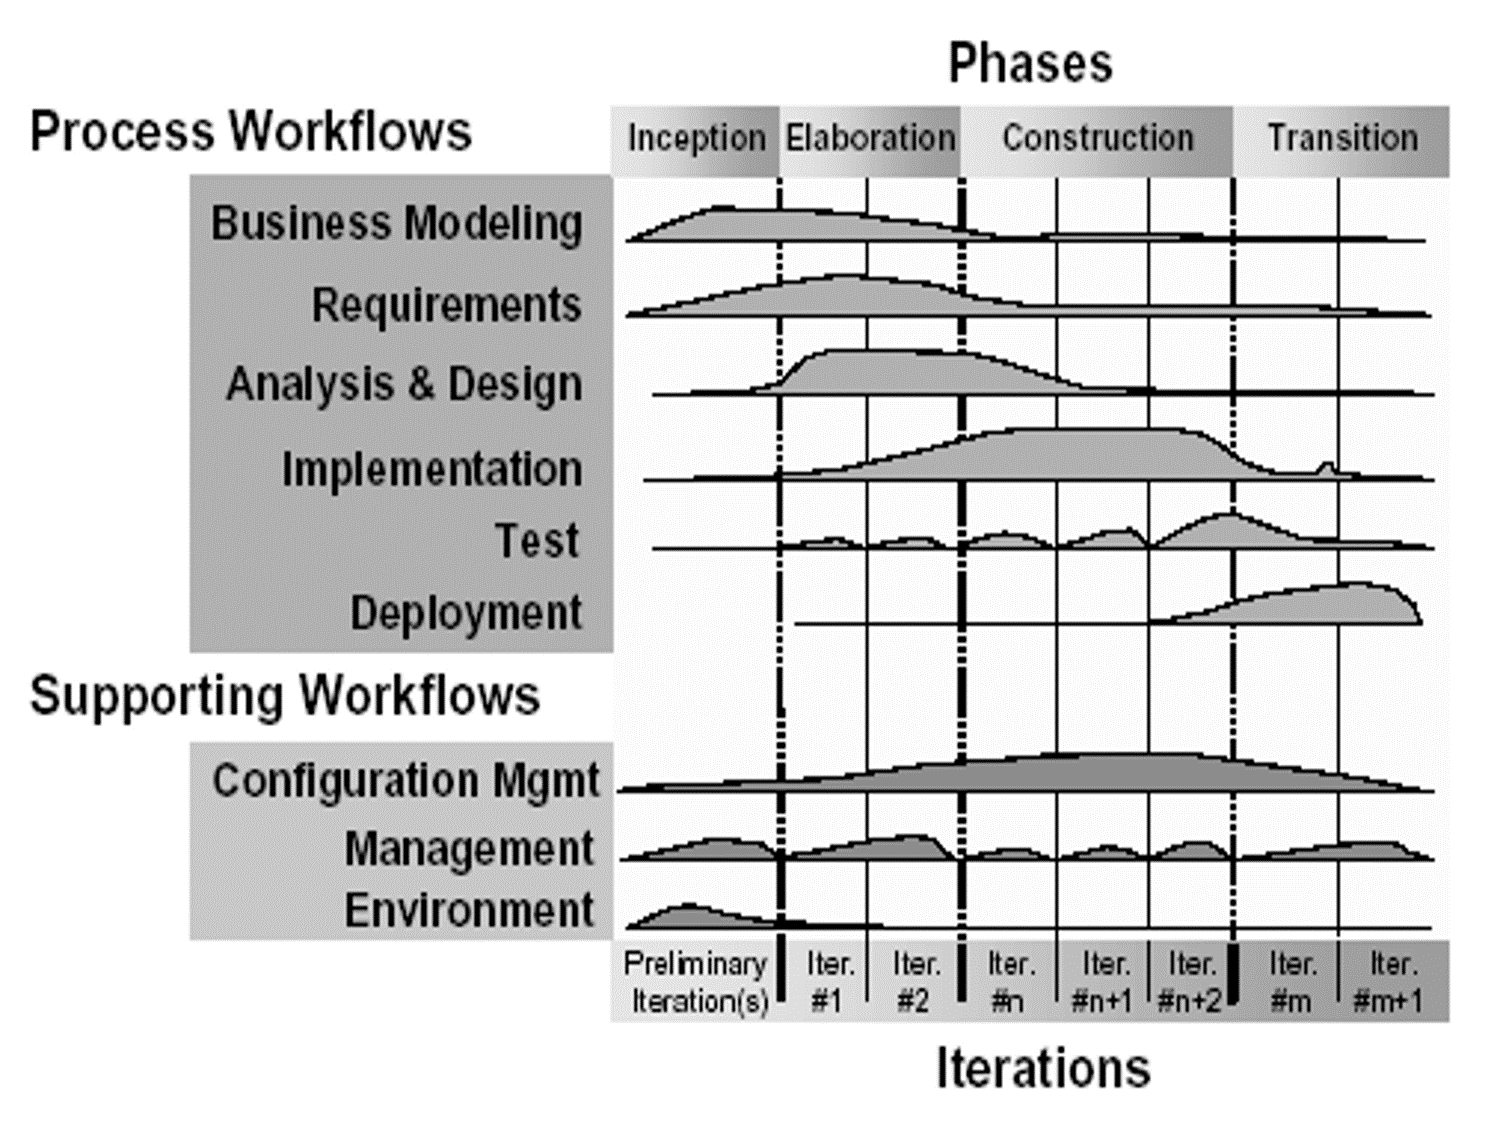
\includegraphics[width=\textwidth, height=\textheight, keepaspectratio]{rup.png}
        \caption{rational unified process}
    \end{figure}
\paragraph{CMM}
\paragraph{SPICE}
\end{document}
